\subsection{Objetivo 2: Integrar el SDK nativo de Estimote con Unity mediante un plugin de comunicación en tiempo real}
Este objetivo tuvo como finalidad establecer la comunicación entre los sensores UWB de Estimote y el entorno Unity, mediante el desarrollo de un módulo nativo en Swift y su integración con la aplicación de realidad aumentada. A través de este proceso se buscó habilitar la adquisición de datos en tiempo real desde el hardware, garantizando su transferencia fluida hacia el motor de visualización y procesamiento.

\subsubsection*{Fase 1: Conexión con sensores UWB}

Durante esta etapa se realizaron múltiples pruebas con los diferentes SDKs oficiales de Estimote. En un principio se experimentó con los SDKs \textit{Indoor Location} y \textit{Proximity}, los cuales en teoría ofrecían funcionalidades equivalentes a un sistema GPS para interiores. Sin embargo, en la práctica ambos presentaron limitaciones técnicas significativas: requerían una configuración extensa, la conexión a los sensores resultaba altamente inestable y el control disponible sobre los dispositivos era insuficiente para los requerimientos de la aplicación. 

El \textit{Proximity SDK} resultaba especialmente prometedor, dado que ofrecía la detección automática de balizas y la generación de eventos de proximidad, pero su comportamiento inconsistente y la limitada documentación disponible lo hicieron inviable para un entorno de desarrollo robusto. Estas pruebas iniciales evidenciaron la necesidad de un enfoque más directo y flexible.

Posteriormente se optó por emplear otro SDK de Estimote que permitía una interacción de menor nivel con los sensores. Este proporcionaba acceso directo a las mediciones de distancia tan pronto como el sensor era descubierto, permitiendo la obtención continua de actualizaciones en tiempo real. A pesar de la mayor libertad que ofrecía, este SDK también presentaba limitaciones importantes: no permitía seleccionar manualmente a qué sensores conectarse, y una vez que un sensor era descubierto, si no se establecía conexión inmediatamente, ya no era posible hacerlo hasta que el sensor se perdiera completamente del rango de detección. Asimismo, aunque el SDK incluía funciones para listar los sensores cercanos, muchas de ellas no funcionaban conforme a la documentación oficial.

% TODO: Aqui esta la fuente para lo del foro (https://forums.estimote.com/t/uwb-beacon-angles/12294)
Una funcionalidad particularmente interesante de este SDK era la posibilidad de obtener, además de la distancia, el ángulo del sensor respecto al dispositivo móvil. Con estos dos valores —distancia y ángulo— sería posible determinar la posición del dispositivo con un único sensor, eliminando la necesidad de trilateración. Sin embargo, esta capacidad solo estaba disponible en un conjunto reducido de dispositivos con múltiples antenas UWB. De acuerdo con la información obtenida en foros de la comunidad de Estimote (ante la escasa documentación oficial), esta función era compatible únicamente con modelos de iPhone 11, 12 y 13. Durante las pruebas se confirmó este comportamiento: un iPhone 12 Mini logró reportar el ángulo correctamente, mientras que modelos más recientes, como el iPhone 14 y 16, no proporcionaban dicha información.

Este hallazgo resultó determinante en el diseño final del sistema. Dado que la obtención del ángulo no era una funcionalidad universal, se descartó el enfoque de posicionamiento basado en un solo sensor y se optó por la trilateración. Esta decisión, aunque más robusta, implicó la necesidad de utilizar al menos tres sensores UWB de manera simultánea, triplicando la cantidad de hardware inicialmente considerada por los antecesores del proyecto.

\newpage
\subsubsection*{Discusión sobre el enfoque previo del proyecto}

Antes de adoptar el nuevo enfoque, se realizó una prueba de concepto basada en la lógica planteada por el equipo previo del megaproyecto. Esta consistía en colocar un único sensor UWB en puntos clave del recorrido —por ejemplo, cruces o intersecciones— con el propósito de guiar al usuario mediante la brújula del dispositivo. La idea era que, al conectarse al sensor más cercano, el sistema pudiera deducir el punto actual del recorrido y orientar al usuario hacia la siguiente dirección.

\begin{figure}[htbp]
  \centering
  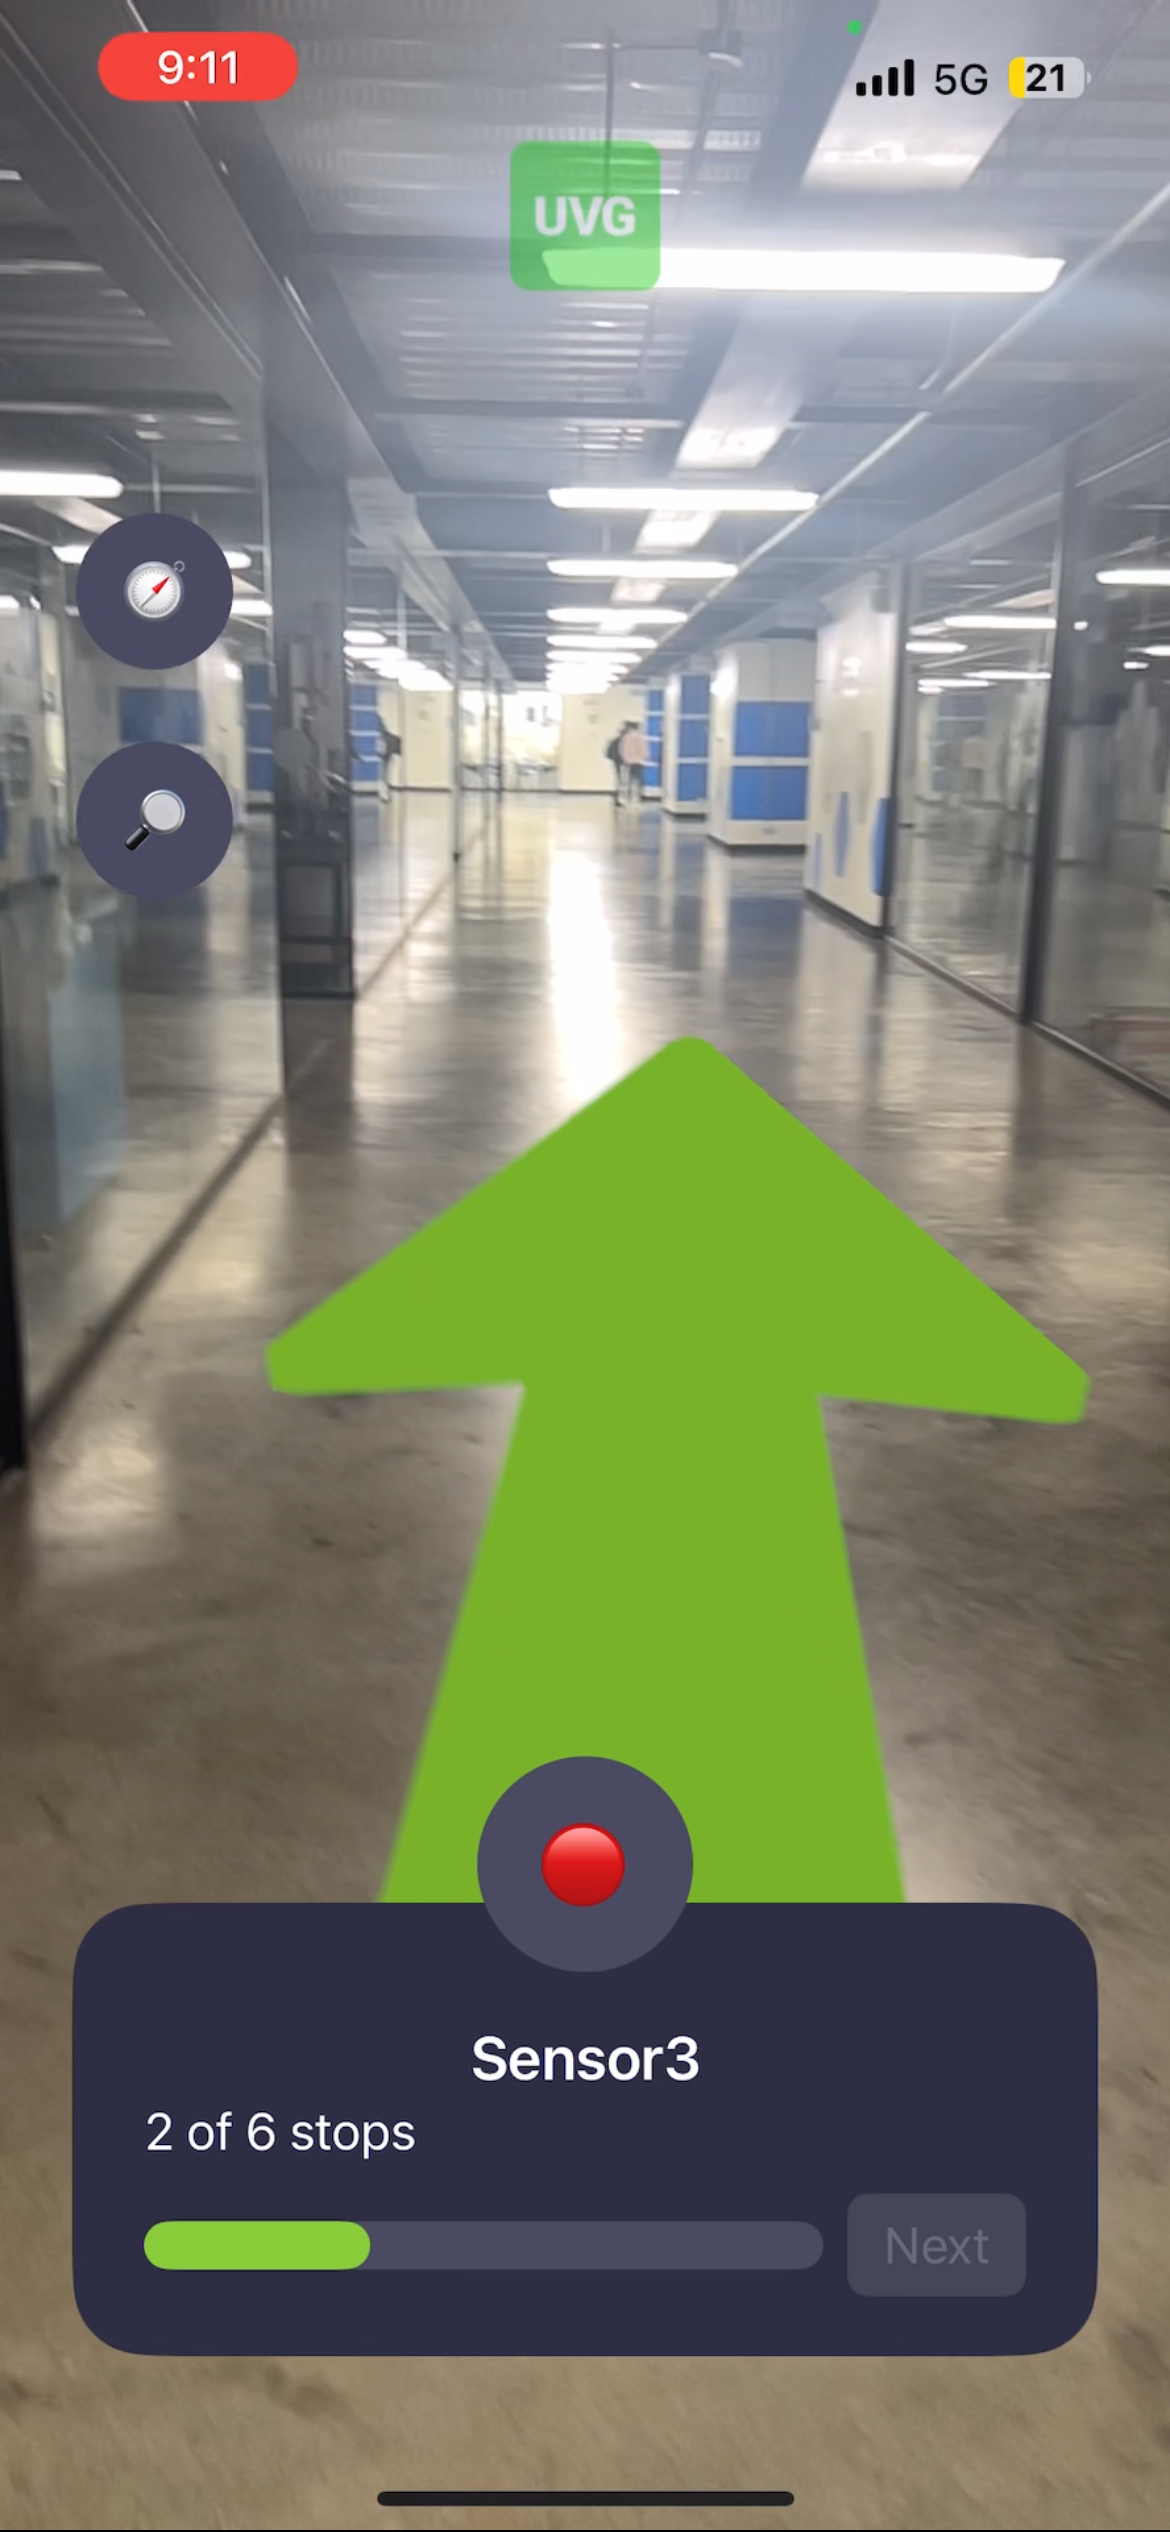
\includegraphics[width=0.2\textwidth]{images/poc_native_swift.PNG}
  \caption{Prueba de concepto con enfoque inicial basada en un solo sensor UWB.}
  \label{fig:poc_native_swift}
\end{figure}

Aunque funcional en escenarios simples, este enfoque presentó múltiples limitaciones para su uso en producción. La conexión con los sensores resultó poco confiable: incluso situando el dispositivo directamente frente al sensor, la conexión podía tardar varios segundos o, en algunos casos, no establecerse en absoluto. A mayores distancias, el problema se agravaba. Además, la escalabilidad del sistema era prácticamente nula, ya que cada nuevo \textit{landmark} agregado requería instalar físicamente un sensor adicional y modificar la capa de software correspondiente. Esto hacía el mantenimiento del sistema costoso y poco sostenible.

Por estas razones, se decidió descartar este enfoque y migrar hacia un sistema basado en trilateración, utilizando tres o más sensores conectados simultáneamente para estimar la posición. Para mitigar los problemas de conexión, se implementó la posibilidad de mantener hasta seis conexiones activas en paralelo, proporcionando redundancia y mayor estabilidad en la adquisición de datos.

\subsubsection*{Fase 2: Desarrollo del plugin nativo para Unity}

Con la comunicación nativa ya establecida, el siguiente paso consistió en desarrollar un plugin que actuara como puente entre Swift (iOS) y Unity. La elección de Unity se basó en su capacidad de ofrecer un entorno multiplataforma, permitiendo construir una sola interfaz visual y mantener únicamente la capa de conexión nativa diferenciada para iOS y Android. 

Antes de integrar el SDK, se realizaron pruebas de viabilidad del plugin. En una primera instancia, se desarrolló una aplicación sencilla en la que Unity invocaba una función en Swift para reproducir un audio, comprobando que las llamadas nativas y la gestión del ciclo de vida del plugin funcionaban correctamente. Posteriormente, se reemplazó el módulo de audio por el SDK de Estimote, verificando que era posible conectar y recibir datos desde Unity, lo que confirmó la factibilidad de este enfoque.

Técnicamente, la integración se realizó exponiendo funciones Swift mediante el sistema de interoperabilidad de Objective-C con Swift, asegurando que fueran públicas para que Unity pudiera reconocerlas en tiempo de ejecución. Este mecanismo permitió que la capa lógica escrita en Swift permaneciera aislada, mientras que Unity se encargaba de visualizar los datos procesados en tiempo real.

\subsubsection*{Fase 3: Validación del flujo de comunicación}

La integración final se validó mediante una escena de prueba en Unity en la que un objeto tridimensional se desplazaba de acuerdo con las coordenadas calculadas por el módulo nativo. En esta arquitectura, Unity ejecuta llamadas periódicas a las funciones expuestas del plugin para obtener los valores más recientes de posición. Dado que la comunicación es unidireccional —de Unity hacia Swift—, no se implementaron mecanismos de notificación inversa. En su lugar, Unity consulta el estado del sistema en cada actualización de cuadro (\textit{frame}), lo cual es suficiente dado el carácter continuo de la actualización de datos.

\begin{figure}[htbp]
  \centering
  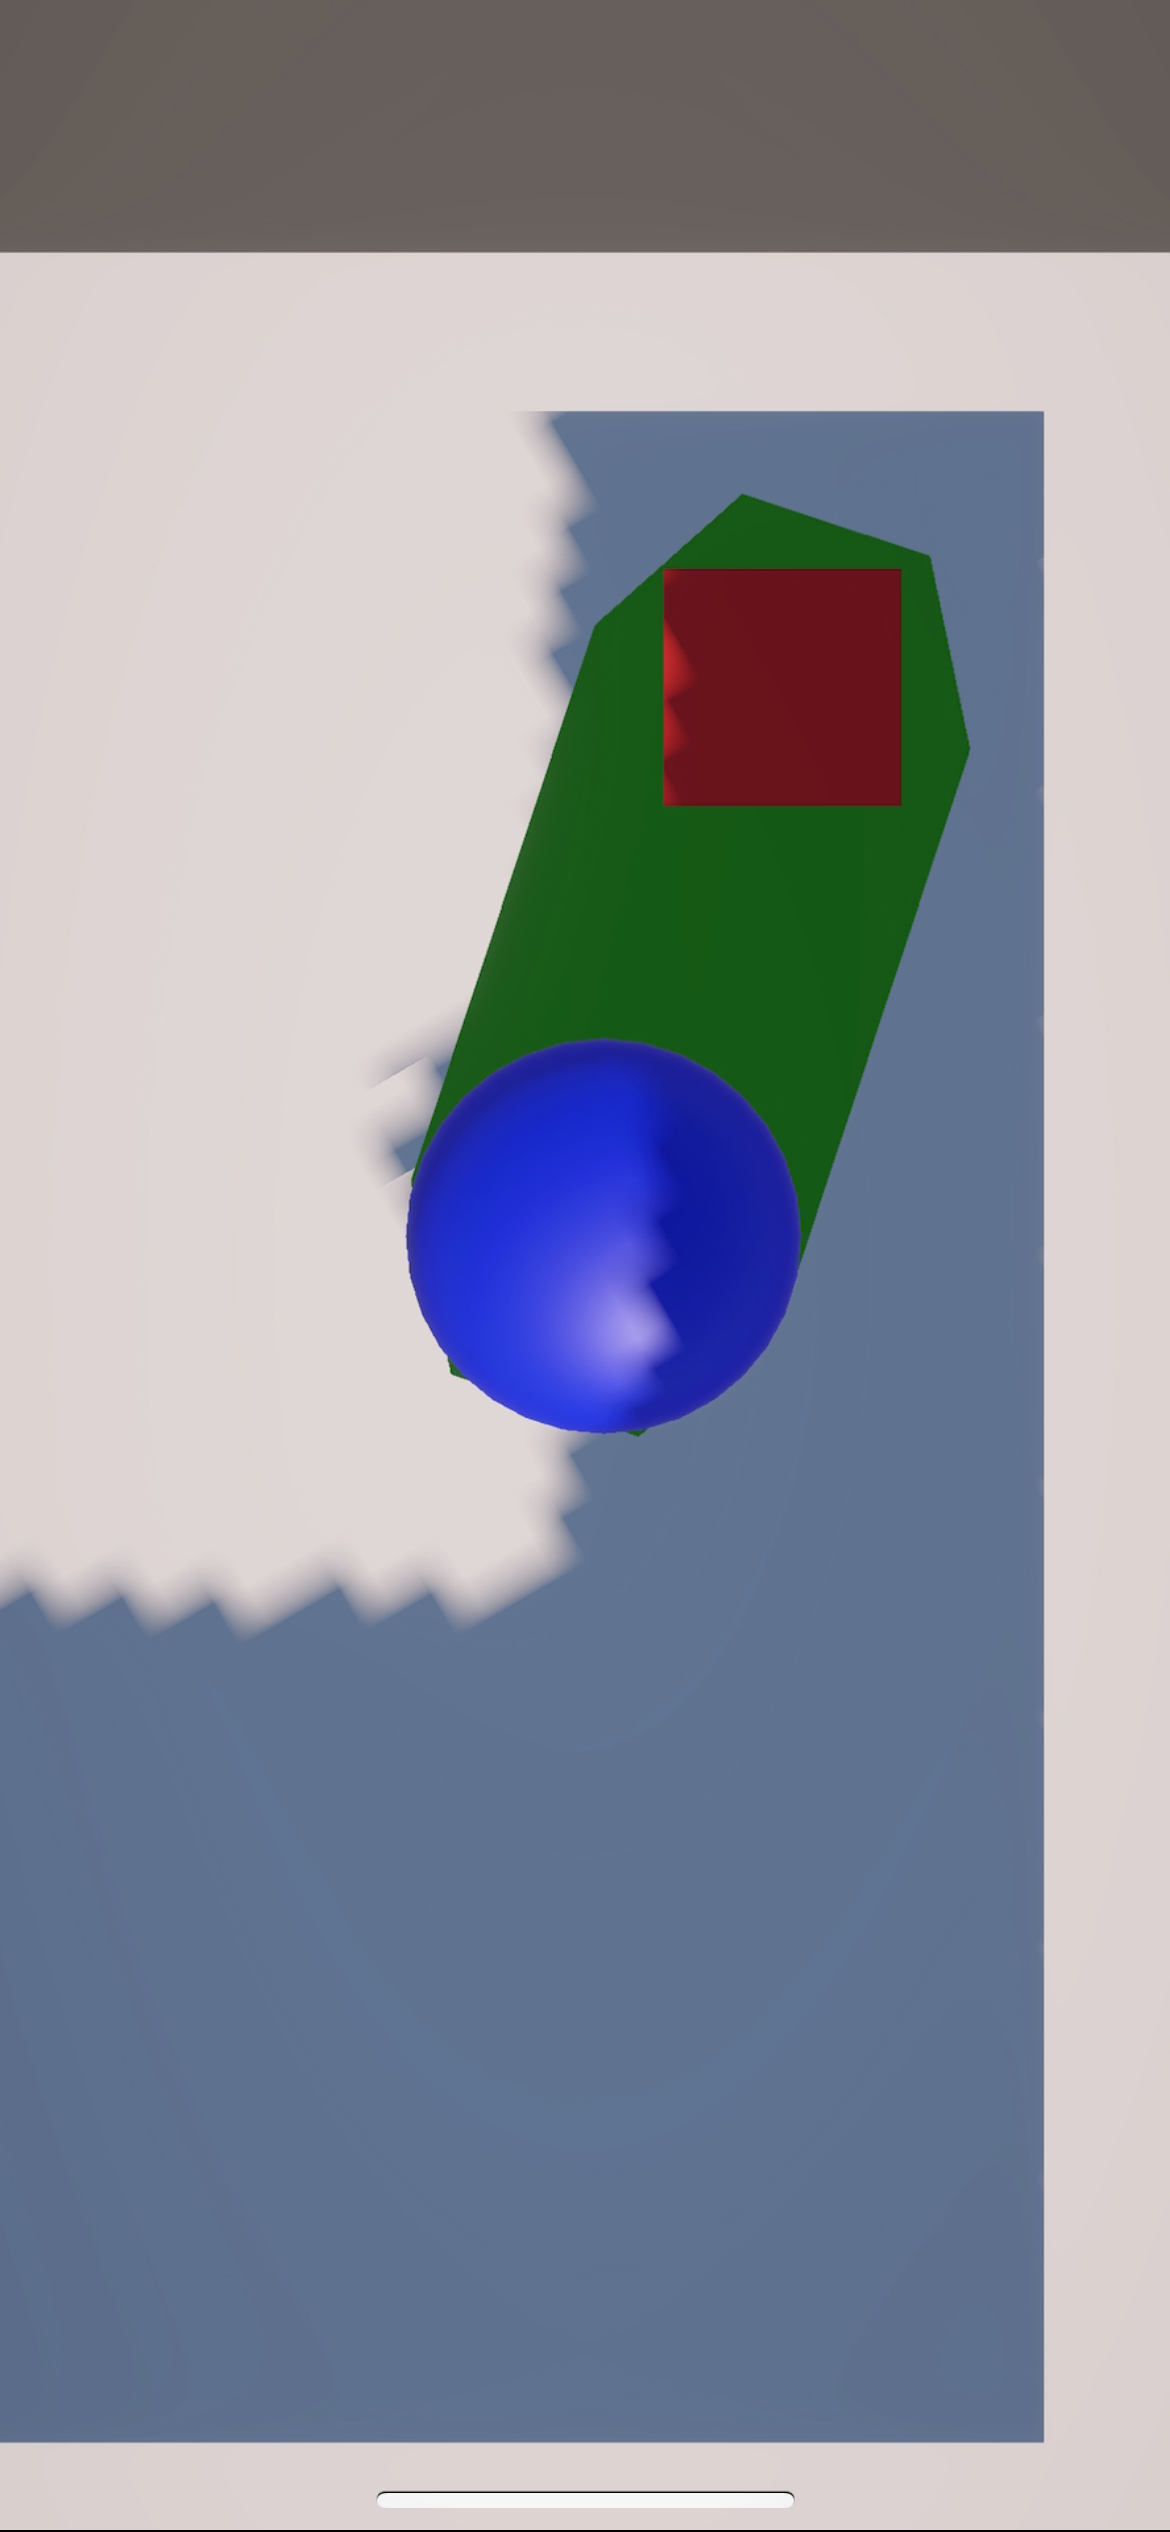
\includegraphics[width=0.2\textwidth]{images/poc_unity.PNG}
  \caption{Prueba de concepto mediante escena de Unity, en azul el objeto tridimensional representando el dispositivo, en verde la ruta que debe seguir el objeto, en rojo la posición de destino.}
  \label{fig:poc_unity}
\end{figure}

Este diseño logró un desempeño fluido e indistinguible de una aplicación nativa, manteniendo frecuencias de actualización sin interrupciones visibles. La comunicación entre el hardware, el módulo nativo y Unity demostró ser estable y de baja latencia, cumpliendo con los requerimientos para la visualización de datos en tiempo real dentro del entorno de realidad aumentada.

% \subsubsection*{Discusión general del objetivo}

% El desarrollo e integración del plugin nativo representó un punto clave en la arquitectura del sistema. A partir de esta infraestructura de comunicación, fue posible conectar la capa de adquisición de datos del hardware con el procesamiento matemático de trilateración y filtrado. La decisión de utilizar Unity permitió consolidar una plataforma escalable y flexible, capaz de integrarse con múltiples tecnologías móviles y extenderse en el futuro hacia Android sin necesidad de rediseñar la interfaz de usuario. 